\documentclass[11pt,a4paper]{article}
\usepackage[margin=2.5cm]{geometry}
\usepackage{amsmath,amssymb}
\usepackage{booktabs}
\usepackage{graphicx}
\usepackage[hidelinks]{hyperref}

\title{Method of manufactured solutions for \texttt{solver2d}\\[0.3em]
\large with the three-equation melt condition at an ice interface}
\date{}

\newcommand{\pd}[2]{\frac{\partial #1}{\partial #2}}

\begin{document}
\maketitle

\section{Purpose}

The method of manufactured solutions (MMS) verifies a code against an exact solution of its own equations.
A smooth function is chosen for every unknown, source terms are added to the equations so that the chosen
functions satisfy them exactly, and the error of the numerical solution is measured on a sequence of grids
and time steps. The observed orders of convergence are then compared with the formal orders of the scheme.

Here the manufactured solution is built so that it satisfies \emph{all} boundary conditions of the ice
set-up of \texttt{solver2d} identically, in particular the nonlinear three-equation melt condition at the
ice and the meltwater velocity at the interface (\texttt{docs/three\_equation\_melt.tex}). The test
therefore covers the velocity--vorticity solver, the scalar solves, the buoyancy, the implicit coupling of
the melt condition to the scalar solves, and the time integration.

\section{Equations and boundary conditions}

\subsection{Equations}

\texttt{solver2d} solves, in non-dimensional form, for the velocity $\mathbf u=(u,v)$, a temperature
$\theta$ and a salinity $s$ on $0\le x<L_x$ (periodic) and $0\le y\le L_y$:
\begin{align}
  \pd{\mathbf u}{t} + (\mathbf u\cdot\nabla)\mathbf u &= -\nabla p + \nu\,\nabla^2\mathbf u
      - \left(Ri_1\,\theta + Ri_2\,s\right)\mathbf e_g + \mathbf f, \qquad \nabla\cdot\mathbf u = 0,
      \label{eq:mom}\\
  \pd{\theta}{t} + \mathbf u\cdot\nabla\theta &= \kappa_T\,\nabla^2\theta + Q_\theta, \label{eq:th}\\
  \pd{s}{t} + \mathbf u\cdot\nabla s &= \kappa_S\,\nabla^2 s + Q_s, \label{eq:s}
\end{align}
with $\nu=1/Re$, $\kappa_T=1/(Re\,Pr)$, $\kappa_S=1/(Re\,Sc)$, the Richardson numbers $Ri_{1,2}$ and the unit
vector $\mathbf e_g=(e_{g,x},e_{g,y})$ in the direction of gravity. $\mathbf f$, $Q_\theta$ and $Q_s$ are the
manufactured source terms (zero in a normal run).

\subsection{Boundary conditions}

\paragraph{\texorpdfstring{Ice at $y=0$}{Ice at y=0}} (no-slip wall with melting, \texttt{bc\_bot = 'noslip'}, \texttt{melt = .true.}).
At every $x$ and $t$, with the interface values $\theta_b=\theta(x,0,t)$, $s_b=s(x,0,t)$ and the melt rate
$m^*$ (a water velocity):
\begin{align}
  \theta_b &= \Lambda\, s_b + \theta_f,                       && \text{liquidus,} \label{eq:liq}\\
  m^* &= St\,\kappa_T\, \pd{\theta}{y}\Big|_{y=0},              && \text{heat balance,} \label{eq:heat}\\
  \kappa_S\,\pd{s}{y}\Big|_{y=0} &= m^*\,(s_b+\sigma),          && \text{salt balance,} \label{eq:salt}\\
  u &= 0, \qquad v = m^*                                       && \text{no slip, meltwater velocity.} \label{eq:vel0}
\end{align}

\paragraph{\texorpdfstring{Wall at $y=L_y$}{Wall at y=Ly}} (\texttt{bc\_top = 'freeslip'}): free slip and fixed scalar values,
\begin{equation}
  \pd{u}{y} = 0, \qquad v = \overline{m^*}(t), \qquad \theta=\theta_{\mathrm{top}}, \qquad s=s_{\mathrm{top}}.
  \label{eq:top}
\end{equation}
The overbar denotes the average over $x$. In 2D the $x$-average of continuity gives
$\partial\bar v/\partial y = 0$, so the mean meltwater velocity is the same at every $y$ and leaves the domain
at $y=L_y$; the fluctuations of $v$ vanish there. In the velocity--vorticity solver the free-slip condition
of the fluctuations is imposed as $\partial^2 v/\partial y^2=0$, which follows from
$\partial u/\partial y=0$ and continuity.

\section{Construction of the manufactured solution}

Throughout, $\eta=y/L_y$, $k_1=2\pi/L_x$ and $\omega=2$.

\subsection{Interface quantities}

The heat and salt balances relate wall gradients to wall values. Instead of solving them, we
\emph{prescribe} the temperature gradient and the salinity at the ice and let the conditions define the
rest:
\begin{align}
  g_T(x,t) &\equiv \pd{\theta}{y}\Big|_{y=0} = A_0(t) + A_1(t)\,\sin k_1 x,
     \qquad A_0 = 1 + \tfrac15\sin\omega t,\quad A_1 = \tfrac{3}{10}\cos\omega t, \\
  s_b(x,t) &= \tfrac12 + \tfrac1{10}\,\sin\!\left(\omega t + \tfrac{3}{10}\right)\cos k_1 x,
\end{align}
and then, from \eqref{eq:liq}--\eqref{eq:salt},
\begin{equation}
  \theta_b = \Lambda\,s_b + \theta_f, \qquad
  m^* = St\,\kappa_T\, g_T, \qquad
  g_S(x,t) \equiv \pd{s}{y}\Big|_{y=0} = \frac{m^*\,(s_b+\sigma)}{\kappa_S}.
  \label{eq:interface}
\end{equation}
With $s_b>0$ and $g_T>0$ the ice melts everywhere ($m^*>0$). The mean melt rate is
$\overline{m^*} = St\,\kappa_T\,A_0(t)$.

\subsection{Scalars}

The scalars are built from three functions of $y$:
\begin{equation}
  \phi_1 = \frac{L_y}{\pi}\sin\pi\eta, \qquad
  \phi_2 = \tfrac12\left(1-\cos\pi\eta\right), \qquad
  \phi_3 = \sin^2\pi\eta ,
\end{equation}
with the properties
\begin{center}
\begin{tabular}{lccc}
\toprule
 & value at $y=0$ & $\partial/\partial y$ at $y=0$ & value at $y=L_y$ \\
\midrule
$\phi_1$ & 0 & 1 & 0 \\
$\phi_2$ & 0 & 0 & 1 \\
$\phi_3$ & 0 & 0 & 0 \\
\bottomrule
\end{tabular}
\end{center}
Then
\begin{align}
  \theta &= \theta_b + g_T\,\phi_1 + (\theta_{\mathrm{top}}-\theta_b)\,\phi_2 + C\,\phi_3,
     & C &= \tfrac15\sin(2k_1x-\omega t), \label{eq:thex}\\
  s      &= s_b + g_S\,\phi_1 + (s_{\mathrm{top}}-s_b)\,\phi_2 + D\,\phi_3,
     & D &= \tfrac1{10}\cos(k_1x+\omega t), \label{eq:sex}
\end{align}
satisfy, by the table, $\theta(x,0,t)=\theta_b$, $\partial_y\theta(x,0,t)=g_T$,
$\theta(x,L_y,t)=\theta_{\mathrm{top}}$, and likewise for $s$. Together with \eqref{eq:interface} the
three-equation condition \eqref{eq:liq}--\eqref{eq:salt} holds at every $x$ and $t$. The terms with
$C\,\phi_3$ and $D\,\phi_3$ add interior structure that does not affect the boundary values. The functions
are trigonometric in $y$, not polynomial, so the compact finite differences do not differentiate them
exactly.

\subsection{Velocity}

A divergence-free velocity is obtained from a stream function $\psi(x,y,t)$, periodic in $x$, plus a
mean flow:
\begin{equation}
  u = U(y,t) + \pd{\psi}{y}, \qquad v = V(t) - \pd{\psi}{x}, \qquad V(t) = \overline{m^*} = St\,\kappa_T\,A_0(t).
\end{equation}
The stream function is
\begin{equation}
  \psi = \Psi_0(x,t)\,a(y) + E(x,t)\,e(y), \qquad
  a = \cos\tfrac{\pi\eta}{2}, \qquad e = \sin\pi\eta\,\sin\tfrac{\pi\eta}{2},
\end{equation}
with
\begin{equation}
  \Psi_0 = \frac{St\,\kappa_T\,A_1(t)}{k_1}\cos k_1 x \quad\Rightarrow\quad
  -\pd{\Psi_0}{x} = St\,\kappa_T\,A_1\sin k_1 x = m^* - \overline{m^*},
\end{equation}
and $E = \tfrac12\sin\!\left(k_1x+\tfrac12\omega t\right)$ adds an interior circulation. The mean flow is
\begin{equation}
  U = \left(1+\tfrac12\sin\omega t\right)\sin\tfrac{\pi\eta}{2}.
\end{equation}
The functions of $y$ have the properties
\begin{center}
\begin{tabular}{lccccc}
\toprule
 & $y=0$ & $\partial_y$ at $y=0$ & $y=L_y$ & $\partial_y$ at $y=L_y$ & $\partial_y^2$ at $y=L_y$ \\
\midrule
$a$ & 1 & 0 & 0 & & 0 \\
$e$ & 0 & 0 & 0 & & 0 \\
$U/U_0$ & 0 & & & 0 & \\
\bottomrule
\end{tabular}
\end{center}
(for $e''(L_y)$: with $e=fg$, $f=\sin\pi\eta$, $g=\sin\frac{\pi\eta}2$, at $\eta=1$ we have $f=f''=0$ and
$g'=0$, so $e''=f''g+2f'g'+fg''=0$). Hence:
\begin{itemize}
  \item at $y=0$: $u = U(0) + \Psi_0 a'(0) + E e'(0) = 0$ and
        $v = V - \partial_x\Psi_0 = \overline{m^*} + (m^*-\overline{m^*}) = m^*$, as required by \eqref{eq:vel0};
  \item at $y=L_y$: $\psi(x,L_y,t)=0$ for all $x$, so $v=V=\overline{m^*}$; and
        $\partial_y u = U'(L_y) + \partial_y^2\psi = 0$, as required by \eqref{eq:top}. The fluctuations
        satisfy $\partial_y^2 v = -\partial_x\partial_y^2\psi = 0$;
  \item $\nabla\cdot\mathbf u = \partial_x\partial_y\psi - \partial_y\partial_x\psi = 0$ everywhere, and
        $\partial_y v = 0$ at $y=0$.
\end{itemize}

\subsection{\texorpdfstring{Fourier content in $x$}{Fourier content in x}}

All fields are trigonometric polynomials in $x$. The highest wavenumber is $2k_1$ in $\theta$ (through $C$)
and in $s$ (through $g_S\propto g_T s_b$); the velocity has wavenumbers up to $k_1$, so the products in the
source terms reach $3k_1$. With
$n_x=16$ Fourier modes these are represented exactly, so the $x$-discretisation contributes no error and
the test measures the wall-normal discretisation, the boundary conditions and the time integration.

\section{Source terms}

Inserting the manufactured fields into \eqref{eq:mom}--\eqref{eq:s} with $p=0$ gives the source terms
\begin{align}
  \mathbf f &= \pd{\mathbf u}{t} + (\mathbf u\cdot\nabla)\mathbf u - \nu\,\nabla^2\mathbf u
               + \left(Ri_1\,\theta + Ri_2\,s\right)\mathbf e_g, \\
  Q_\theta &= \pd{\theta}{t} + \mathbf u\cdot\nabla\theta - \kappa_T\nabla^2\theta, \qquad
  Q_s = \pd{s}{t} + \mathbf u\cdot\nabla s - \kappa_S\nabla^2 s .
\end{align}
The pressure is then zero. \texttt{solver2d} uses the rotational form $\mathbf u\times\boldsymbol\omega$ of
the nonlinear term, which differs from $-(\mathbf u\cdot\nabla)\mathbf u$ by the gradient
$\nabla(|\mathbf u|^2/2)$. That gradient is absorbed into the (total) pressure: the velocity--vorticity
solver uses only the curl of the momentum equation, and the $x$-average of the $x$-component of a gradient
of a periodic function vanishes. The manufactured velocity is therefore an exact solution for either form.

The derivatives are taken symbolically with sympy (\texttt{tools/mms/mms\_solution.py}), which also checks
that all boundary conditions and continuity hold identically, and writes the Fortran module
\texttt{src/mms\_solution.f90} (with common-subexpression elimination) for the fields, the source terms and
the interface values. The parameters $\nu$, $\kappa_T$, $\kappa_S$, $Ri_{1,2}$, $\mathbf e_g$, $St$, $\Lambda$,
$\theta_f$, $\sigma$, $L_x$, $L_y$, $\theta_{\mathrm{top}}$, $s_{\mathrm{top}}$ are arguments, taken from the input
at run time.

\section{Use in the code}

With \texttt{mms = .true.} in \texttt{\&mms\_test}, \texttt{solver2d}
\begin{enumerate}
  \item starts from the manufactured fields at $t=0$, evaluated on the dealiased physical grid and
        transformed to Fourier space (the initial error is at round-off);
  \item adds $\mathbf f$, $Q_\theta$, $Q_s$, evaluated on the physical grid and transformed, to the explicit
        terms of each Runge--Kutta substep. The low-storage RK3 of Spalart, Moser \& Rogers evaluates its
        explicit terms at the stage times $t_q = t + c_q\Delta t$ with
        \begin{equation*}
          c_1 = 0,\qquad c_2 = \gamma_1 = \tfrac{8}{15},\qquad
          c_3 = \gamma_1 + \gamma_2 + \zeta_2 = \tfrac8{15} + \tfrac5{12} - \tfrac{17}{60} = \tfrac23 ;
        \end{equation*}
  \item imposes the melt condition and $v=m^*$ at $y=0$ exactly as in a normal run;
  \item writes \texttt{data/mms\_error.dat} at every log step: the maximum over the physical grid of
        $|u-u_{\mathrm{ex}}|$, $|v-v_{\mathrm{ex}}|$, $|\theta-\theta_{\mathrm{ex}}|$, $|s-s_{\mathrm{ex}}|$, and at the
        ice the errors of $m^*$ ($=v$ there), $\theta_b$ and $s_b$.
\end{enumerate}

\section{Results}

Parameters (\texttt{examples/mms/input.nml}): $L_x=2$, $L_y=1$, $n_x=16$, $Re=100$, $Pr=1$, $Sc=2$,
$St=5$, $\Lambda=-0.5$, $\theta_f=0.2$, $\sigma=0.3$, $\theta_{\mathrm{top}}=s_{\mathrm{top}}=1$,
$Ri_1=0.1$, $Ri_2=-0.05$, gravity along $(0.3,1)$, Crank--Nicolson for the scalar diffusion, grid refined at the
ice (\texttt{tanh\_bot}, $\alpha_s=2$), $t=0$ to $0.5$. The study is run with
\texttt{python3 convergence.py} in \texttt{examples/mms}.

\paragraph{Space.} $n_y = 17,\dots,257$ at $\Delta t = 5\times10^{-4}$ (the time error is negligible):
maximum errors at $t=0.5$, and the observed orders $\log_2[e(h)/e(h/2)]$ between successive grids.
\begin{center}
\small
\begin{tabular}{rccccccc}
\toprule
$n_y$ & $u$ & $v$ & $\theta$ & $s$ & $m^*$ & $\theta_b$ & $s_b$ \\
\midrule
 17 & 1.50e-2 & 5.91e-3 & 1.15e-3 & 1.35e-2 & 2.93e-5 & 1.26e-4 & 2.53e-4 \\
 33 & 1.89e-3 & 7.45e-4 & 1.16e-4 & 1.69e-3 & 3.06e-6 & 1.21e-5 & 2.41e-5 \\
 65 & 2.53e-4 & 9.85e-5 & 1.41e-5 & 2.21e-4 & 3.52e-7 & 1.30e-6 & 2.61e-6 \\
129 & 3.27e-5 & 1.26e-5 & 1.76e-6 & 2.80e-5 & 4.23e-8 & 1.52e-7 & 3.03e-7 \\
257 & 4.17e-6 & 1.58e-6 & 2.20e-7 & 3.51e-6 & 6.53e-9 & 1.84e-8 & 3.69e-8 \\
\midrule
\multicolumn{8}{l}{observed order} \\
17--33   & 2.99 & 2.99 & 3.31 & 2.99 & 3.26 & 3.39 & 3.39 \\
33--65   & 2.90 & 2.92 & 3.05 & 2.93 & 3.12 & 3.21 & 3.21 \\
65--129  & 2.95 & 2.97 & 3.00 & 2.98 & 3.05 & 3.10 & 3.10 \\
129--257 & 2.97 & 3.00 & 3.00 & 3.00 & 2.70 & 3.04 & 3.04 \\
\bottomrule
\end{tabular}
\end{center}

\paragraph{Time.} $n_y=65$, $\Delta t = 0.016,\dots,0.002$, $t=0$ to $0.48$. The spatial error is much
larger than the temporal error on any affordable grid, so the temporal error is measured against a run with
$\Delta t = 2.5\times10^{-4}$ on the same grid, in which the spatial error is the same and cancels: maximum
differences of the Fourier coefficients.
\begin{center}
\small
\begin{tabular}{rccccc}
\toprule
$\Delta t$ & $u$ & $v$ & $\theta$ & $s$ & $m^*$ \\
\midrule
0.016 & 9.19e-7 & 5.62e-7 & 1.07e-6 & 2.35e-6 & 1.24e-7 \\
0.008 & 1.16e-7 & 1.06e-7 & 1.45e-7 & 4.53e-7 & 1.06e-7 \\
0.004 & 2.55e-8 & 3.75e-8 & 2.12e-8 & 1.06e-7 & 3.75e-8 \\
0.002 & 6.58e-9 & 1.06e-8 & 4.88e-9 & 2.52e-8 & 1.06e-8 \\
\midrule
\multicolumn{6}{l}{observed order} \\
0.016--0.008 & 2.98 & 2.41 & 2.89 & 2.38 & 0.23 \\
0.008--0.004 & 2.19 & 1.50 & 2.77 & 2.10 & 1.50 \\
0.004--0.002 & 1.95 & 1.83 & 2.12 & 2.07 & 1.83 \\
\bottomrule
\end{tabular}
\end{center}
At the largest time step the melt rate $m^*$ is less sensitive to $\Delta t$ than the fields; from
$\Delta t=0.008$ on its difference equals that of $v$, whose maximum lies at the ice.

\begin{figure}[h]
  \centering
  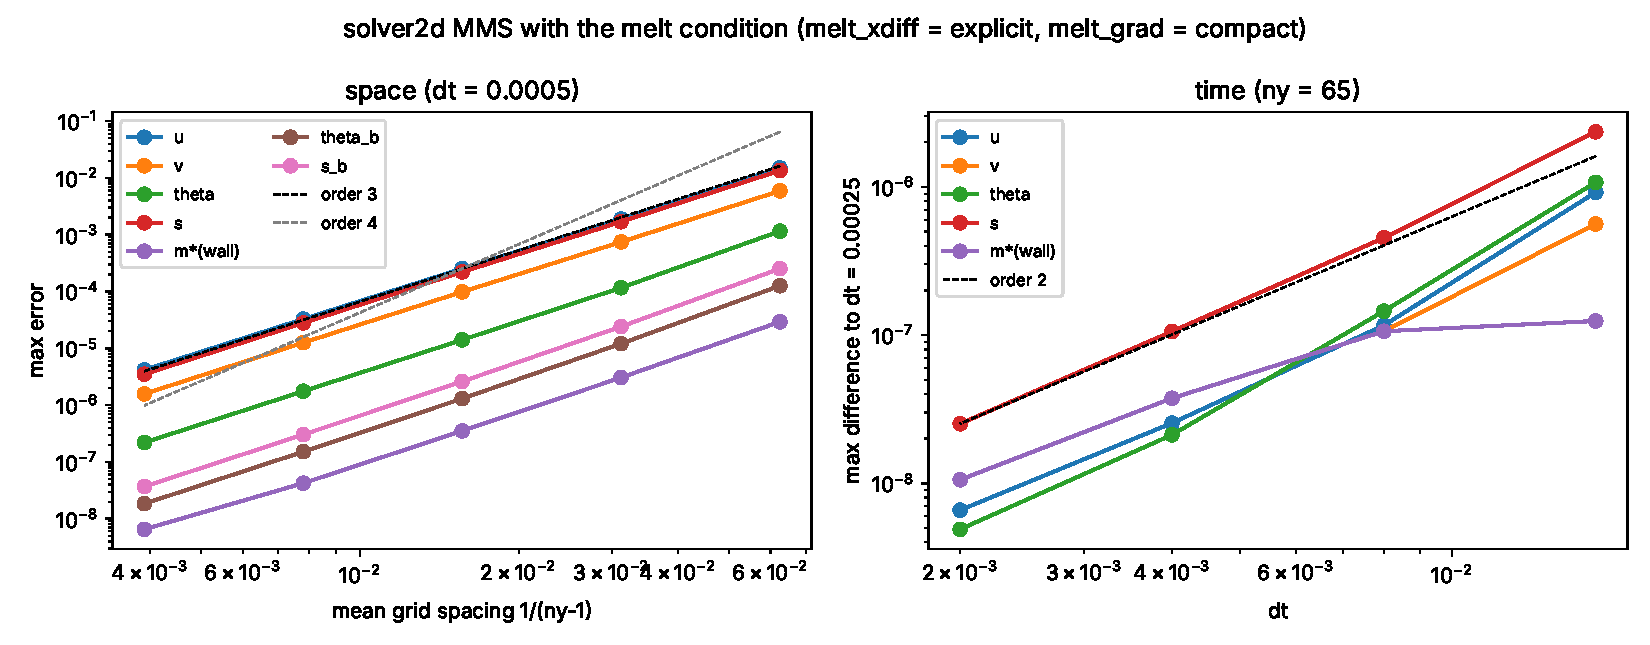
\includegraphics[width=\textwidth]{mms_convergence.pdf}
  \caption{Convergence of the manufactured solution: space (left, $\Delta t=5\times10^{-4}$) and time
  (right, $n_y=65$, differences to $\Delta t=2.5\times10^{-4}$).}
  \label{fig:conv}
\end{figure}

\section{Discussion}

\begin{itemize}
  \item \textbf{Time.} All quantities converge at second order as $\Delta t$ decreases, the order of the
        Crank--Nicolson treatment of the diffusion (the explicit terms are third order; this shows at the
        largest time steps).
  \item \textbf{Space.} All fields, and the melt rate and interface values at the ice, converge at third
        order. The sixth-order compact scheme (3-5-6-5-3) has third-order closures at the boundary rows, and
        these set the global order. The melt condition is not the limiting factor: with a fifth-order
        one-sided wall gradient in the melt condition (\texttt{melt\_grad = 'explicit'}) the interface
        values are 3--7 times more accurate on the coarser grids, but the errors of $u$, $v$, $\theta$ and $s$
        are unchanged to three digits, and on the finest grid both choices give the same melt-rate error.
  \item \textbf{Couplings.} The exact one-pass coupling (\texttt{melt\_xdiff = 'explicit'}) and the
        iterative one (\texttt{'implicit'}) give nearly identical errors and the same orders.
  \item \textbf{Consistency.} The results are bit-identical on 1 and 3 MPI ranks, and the OpenACC code path
        (host build) agrees to $1.5\times10^{-13}$.
\end{itemize}

\end{document}
